\documentclass[12pt,letterpaper]{exam}
\usepackage[lmargin=1in,rmargin=1in,tmargin=1in,bmargin=1in]{geometry}
\usepackage{../style/exams}

% -------------------
% Course & Exam Information
% -------------------
\newcommand{\course}{MAT 101: Exam 3}
\newcommand{\term}{Spring -- 2022}
\newcommand{\examdate}{05/12/2022}
\newcommand{\timelimit}{85 Minutes}

\setbool{hideans}{true} % Student: True; Instructor: False

% -------------------
% Content
% -------------------
\begin{document}

\examtitle
\instructions{Write your name on the appropriate line on the exam cover sheet. This exam contains \numpages\ pages (including this cover page) and \numquestions\ questions. Check that you have every page of the exam. Answer the questions in the spaces provided on the question sheets. Be sure to answer every part of each question and show all your work.} 
\scores
%\bottomline
\newpage

% ---------
% Questions
% ---------
\begin{questions}

% Question 1
\newpage
\question Compute the functions at the indicated value below. Your answers should be exact. \pspace

\begin{parts}
\part[2] $f(x)= -4(5^x)$ \vfill
	\[
	f(2)= \hspace{9cm}
	\] \vfill

\part[2] $g(x)= 5(2^x)$ \vfill
	\[
	g(0)= \hspace{9cm}
	\] \vfill

\part[2] $h(x)= -6(4^{1 - 2x})$ \vfill
	\[
	h(1)= \hspace{9cm}
	\] \vfill

\part[2] $r(x)= 7 \left( \dfrac{3}{5} \right)^x$ \vfill
	\[
	r(-2)= \hspace{9cm}
	\] \vfill

\part[2] $s(x)= 8(9^x)$ \vfill
	\[
	s \left( -\frac{1}{2} \right)= \hspace{8.8cm}
	\]
\end{parts}



% Question 2
\newpage
\question Using exact values, write the following functions in the form $y= Ab^x$: \pspace

\begin{parts}
\part[3] $f(x)= -5(3^{2x})$ \vfill

\part[3] $g(x)= 3 \left( \dfrac{5}{7} \right)^{-x}$ \vfill

\part[4] $h(x)= 5 (2^{1 - 3x})$ \vfill
\end{parts}



% Question 3
\newpage
\question Determine whether the following functions are increasing or decreasing: \pspace

\begin{parts}
\part[3] $f(x)= 3 \left( \dfrac{10}{11} \right)^x$ \vfill

\part[3] $g(x)= 17 (5^{-2x})$ \vfill

\part[4] $h(x)= -9 \left( \dfrac{7}{5} \right)^{2 - x}$ \vfill
\end{parts}



% Question 4
\newpage
\question[10] Sketch the function $y= -2 \left( \dfrac{1}{3} \right)^{x - 1}$ on the graph below. 
	\[
	\fbox{
	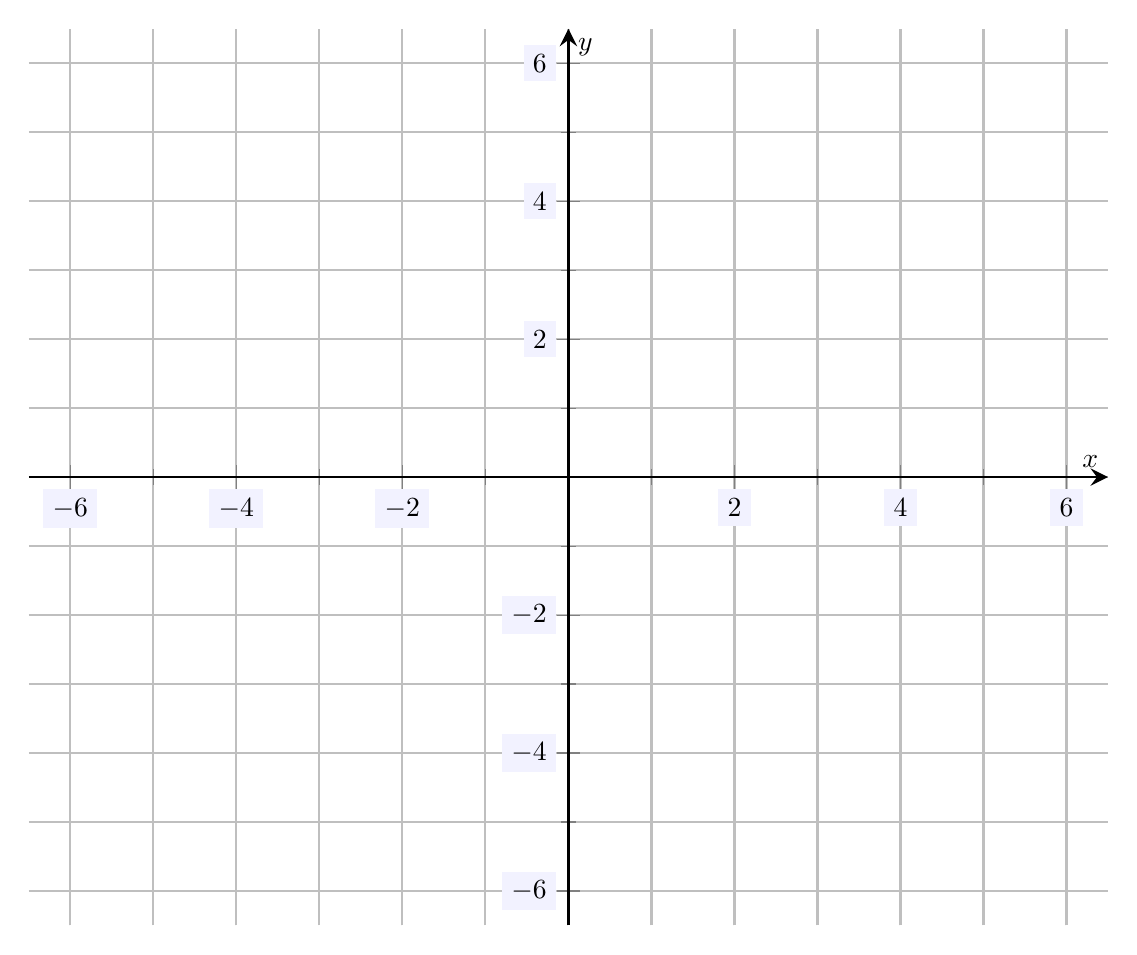
\begin{tikzpicture}[scale=2,every node/.style={scale=0.5}]
	\begin{axis}[
	grid=both,
	axis lines=middle,
	ticklabel style={fill=blue!5!white},
	xmin= -6.5, xmax=6.5,
	ymin= -6.5, ymax=6.5,
	xtick={-6,-4,-2,0,2,4,6},
	ytick={-6,-4,-2,0,2,4,6},
	minor tick = {-7,-6,...,7},
	xlabel=\(x\),ylabel=\(y\),
	]
	\end{axis}
	\end{tikzpicture}
	}
	\]



% Question 5
\newpage
\question[10] Find the exact values of the following: \pspace

\begin{enumerate}[(a)]
\item $\log_3 3^{2022}$ \vfill

\item $\log_6 \left( \dfrac{1}{6^{1995}} \right)$ \vfill

\item $\log_7 1$ \vfill

\item $\ln(e^{10/11})$ \vfill

\item $\log_2(64)$ \vfill
\end{enumerate}



% Question 6
\newpage
\question[10] Write the following as a single logarithm involving no negative powers:
	\[
	5 \log_3(x) - 2 \log_3(y) - 6 \log_3(z^{-1}) + 4
	\]



% Question 7
\newpage
\question[10] Write the following in terms of $\ln x$, $\ln y$, and $\ln z$:
	\[
	\ln \left( \dfrac{x^{10}}{y^{-5} z^7} \right)
	\]



% Question 8
\newpage
\question[10] Use the change of base formula to convert $\log_8(4)$ to base-2 and then find the exact value. 



% Question 9
\newpage
\question Complete the following:

\begin{parts}
\part[5] How many digits does $2021^{2022}$ have in base-10? \vfill

\part[5] How many digits does $2021^{2022}$ have in base-8? \vfill
\end{parts}



% Question 10
\newpage
\question[10] Is there a whole number $k$ such that $2022^k$ has 15,000 digits? Explain.



% Question 11
\newpage
\question[10] Showing all your work, find the exact solution to the following: 
	\[
	\dfrac{1}{25^x} - 4= 1
	\]



% Question 12
\newpage
\question[10] Showing all your work, find the exact solution to the following:  
	\[
	15 - \log_2(4 - x)= 10
	\]



% Question 13
\newpage
\question[10] Showing all your work, find the exact solution to the following: 
	\[
	e^{x/3} + 12= 20
	\]



% Question 14
\newpage
\question[10] Showing all your work, find the exact solution to the following: 
	\[
	\ln(3x) + 10= 8
	\]



% Question 15
\newpage
\question[10] Showing all your work, find the exact solution to the following: 
	\[
	3\left( \dfrac{1}{2} \right)^{5x + 3}= 45
	\]



% Question 16
\newpage
\question[10] Showing all your work, find the exact solution to the following: 
	\[
	3 - \log_2(x)= \log_2(x + 2)
	\]



% Question 17
\newpage
\question[10] Suppose Alice invests \$5,000 into an account which earns 4.5\% annual interest, compounded monthly. How much will the investment be worth in 8~years? How much interest has been earned during this time period? 



% Question 18
\newpage
\question[10] Bob takes out a \$750 loan with an interest rate of 6.4\%, compounded continuously. Supposing the loan ends after two and a half years, how much does Bob owe after this time? How much total interest does he pay on this loan?



% Question 19
\newpage
\question[10] Suppose Montez takes out a loan to expand his small business. The loan is for \$25,000 at a 3.8\% annual interest rate, compounded quarterly. How long until the amount of money he owes on the loan has doubled?



% Question 20
\newpage
\question[10] Jillian buys \$900 in a stock which promises annual returns of 1.3\%, compounded continuously. How long does Jillian have to wait until this stock is worth \$1,500?


\end{questions}
\end{document}